\documentclass{article}

% packages
\usepackage{amsmath, amsthm, thmtools, amsfonts, amssymb, luacode, catchfile, tikzducks, hyperref, ifthen}
\ifcsname c@kobocompile\endcsname
	\usepackage[a5paper, total={1072pt, 1448pt}, margin=10pt, includeheadfoot]{geometry} % set page margins
\else
	\usepackage[a4paper, margin=50pt, includeheadfoot]{geometry}
\fi
\usepackage[shortlabels]{enumitem}
\usepackage[skip=3pt, indent=0pt]{parskip}

% language
\usepackage[bidi=basic, layout=tabular, provide=*]{babel}
\ifcsname c@english\endcsname
	\babelprovide[main, import]{english}
\else
	\babelprovide[main, import]{hebrew}
	\babelprovide{rl}
\fi
%\babelfont{rm}{Libertinus Serif}
\babelfont{rm}[Renderer=Harfbuzz]{Libertinus Serif}
\babelfont{sf}{Libertinus Sans}
\babelfont{tt}{Libertinus Mono}

% style
\AddToHook{cmd/section/before}{\clearpage}	% Add line break before section
\linespread{1.3}
\setcounter{secnumdepth}{0}		% Remove default number tags from sections, this won't do well with theorems
\AtBeginDocument{\setlength{\belowdisplayskip}{3pt}}
\AtBeginDocument{\setlength{\abovedisplayskip}{3pt}}
\graphicspath{ {../images/} }

% operators
\DeclareMathOperator\cis{cis}
\DeclareMathOperator\Sp{Sp}
\DeclareMathOperator\tr{tr}
\DeclareMathOperator\im{Im}
\DeclareMathOperator\re{Re}
\DeclareMathOperator\diag{diag}
\DeclareMathOperator*\lowlim{\underline{lim}}
\DeclareMathOperator*\uplim{\overline{lim}}
\DeclareMathOperator\rng{rng}
\DeclareMathOperator\Sym{Sym}
\DeclareMathOperator\Arg{Arg}
\DeclareMathOperator\Log{Log}
\DeclareMathOperator\dom{dom}
\DeclareMathOperator\supp{Supp}
\DeclareMathOperator\var{Var}
\DeclareMathOperator\cov{Cov}

% commands
%\renewcommand\qedsymbol{\textbf{מש''ל}}
%\renewcommand\qedsymbol{\fbox{\emoji{lizard}}}
\newcommand{\Aa}[0]{\mathcal{A}}
\newcommand{\Bb}[0]{\mathcal{B}}
\newcommand{\CC}[0]{\mathbb{C}}
\newcommand{\Cc}[0]{\mathcal{C}}
\newcommand{\EE}[0]{\mathbb{E}}
\newcommand{\FF}[0]{\mathbb{F}}
\newcommand{\Ff}[0]{\mathcal{F}}
\newcommand{\Ii}[0]{\mathcal{I}}
\newcommand{\Gg}[0]{\mathcal{G}}
\newcommand{\Ll}[0]{\mathcal{L}}
\newcommand{\Mm}[0]{\mathcal{M}}
\newcommand{\NN}[0]{\mathbb{N}}
\newcommand{\Nn}[0]{\mathcal{N}}
\newcommand{\PP}[0]{\mathbb{P}}
\newcommand{\Pp}[0]{\mathcal{P}}
\newcommand{\QQ}[0]{\mathbb{Q}}
\newcommand{\RR}[0]{\mathbb{R}}
\newcommand{\Rr}[0]{\mathcal{R}}
\newcommand{\Ss}[0]{\mathcal{S}}
\newcommand{\TT}[0]{\mathbb{T}}
\newcommand{\Uu}[0]{\mathcal{U}}
\newcommand{\Vv}[0]{\mathcal{V}}
\newcommand{\Ww}[0]{\mathcal{W}}
\newcommand{\ZZ}[0]{\mathbb{Z}}
\newcommand{\acts}[0]{\circlearrowright}
\newcommand{\explain}[2] {
	\begin{flalign*}
		 && \text{#2} && \text{#1}
	\end{flalign*}
}
\newcommand{\maketitleprint}[0]{ \begin{center}
	%\begin{tikzpicture}[scale=3]
	%	\duck[graduate=gray!20!black, tassel=red!70!black]
	%\end{tikzpicture}	
	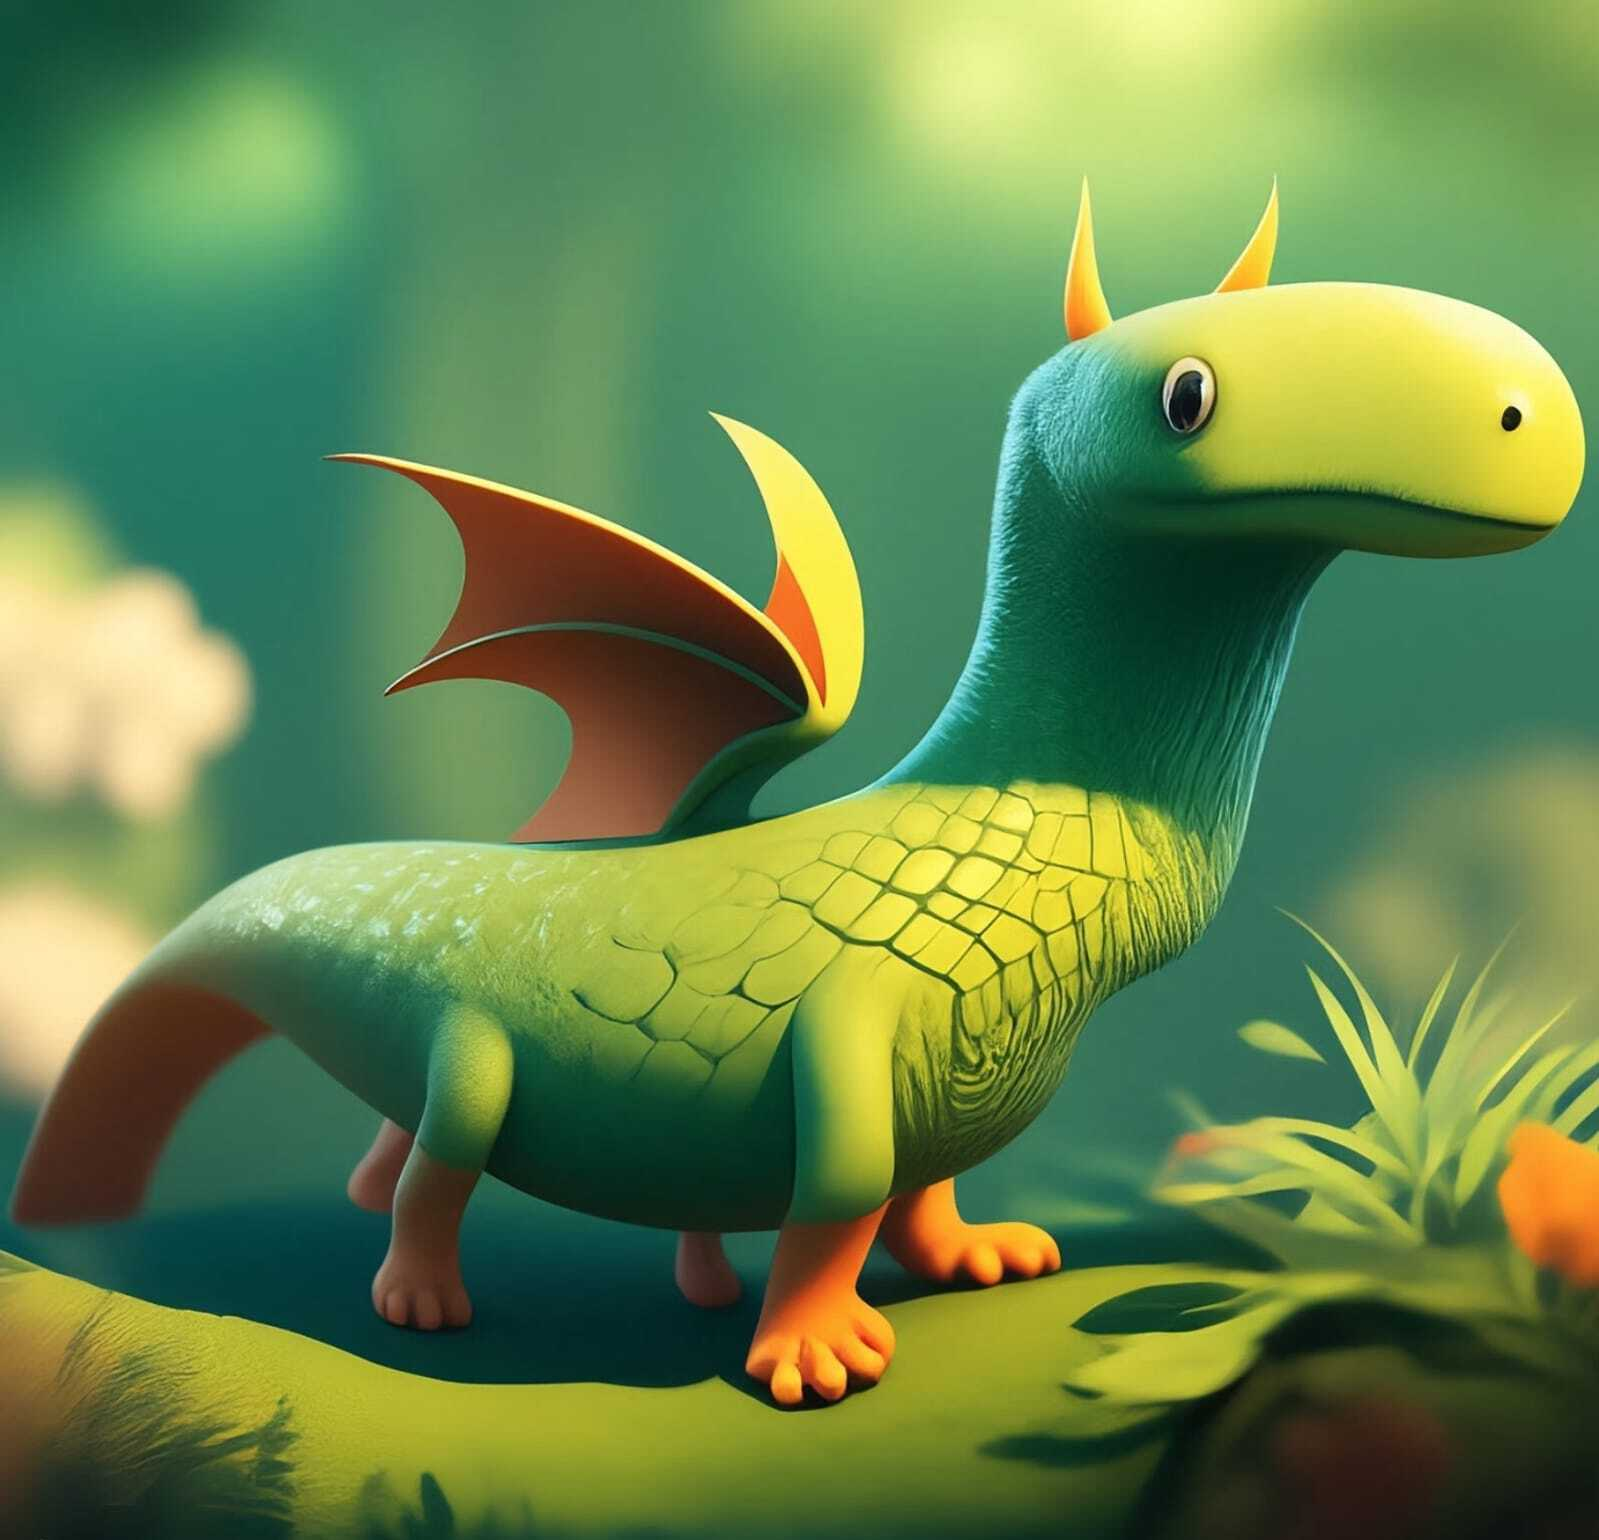
\includegraphics[width=6cm]{cover}
\end{center}
}

% theorem commands
\newtheoremstyle{c_remark}
	{}	% Space above
	{}	% Space below
	{}% Body font
	{}	% Indent amount
	{\bfseries}	% Theorem head font
	{}	% Punctuation after theorem head
	{.5em}	% Space after theorem head
	{\thmname{#1}\thmnumber{ #2}\thmnote{ \normalfont{\text{(#3)}}}}	% head content
\newtheoremstyle{c_definition}
	{3pt}	% Space above
	{3pt}	% Space below
	{}% Body font
	{}	% Indent amount
	{\bfseries}	% Theorem head font
	{}	% Punctuation after theorem head
	{.5em}	% Space after theorem head
	{\thmname{#1}\thmnumber{ #2}\thmnote{ \normalfont{\text{(#3)}}}}	% head content
\newtheoremstyle{c_plain}
	{3pt}	% Space above
	{3pt}	% Space below
	{\itshape}% Body font
	{}	% Indent amount
	{\bfseries}	% Theorem head font
	{}	% Punctuation after theorem head
	{.5em}	% Space after theorem head
	{\thmname{#1}\thmnumber{ #2}\thmnote{ \text{(#3)}}}	% head content

\ifcsname c@english\endcsname
	\theoremstyle{plain}
	\newtheorem{theorem}{Theorem}[section]
	\newtheorem{lemma}[theorem]{Lemma}
	\newtheorem{proposition}[theorem]{Proposition}
	\newtheorem*{proposition*}{Proposition}
	%\newtheorem{corollary}[theorem]{אין חלופה עברית}

	\theoremstyle{definition}
	\newtheorem{definition}[theorem]{Definition}
	\newtheorem*{definition*}{Definition}
	\newtheorem{example}{Example}[section]
	\newtheorem{exercise}{Exercise}[section]

	\theoremstyle{remark}
	\newtheorem*{remark}{Remark}
	\newtheorem*{solution}{Solution}
	\newtheorem{conclusion}[theorem]{Conclusion}
	\newtheorem{notation}[theorem]{Notation}
\else
	\theoremstyle{c_plain}
	\newtheorem{theorem}{משפט}[section]
	\newtheorem{lemma}[theorem]{למה}
	\newtheorem{proposition}[theorem]{טענה}
	\newtheorem*{proposition*}{טענה}
	%\newtheorem{corollary}[theorem]{אין חלופה עברית}

	\theoremstyle{c_definition}
	\newtheorem{definition}[theorem]{הגדרה}
	\newtheorem*{definition*}{הגדרה}
	\newtheorem{example}{דוגמה}[section]
	\newtheorem{exercise}{תרגיל}[section]

	\theoremstyle{c_remark}
	\newtheorem*{remark}{הערה}
	\newtheorem*{solution}{פתרון}
	\newtheorem{conclusion}[theorem]{מסקנה}
	\newtheorem{notation}[theorem]{סימון}
\fi

% Questions related commands
\newcounter{question}
\setcounter{question}{1}
\newcounter{sub_question}
\setcounter{sub_question}{1}

\ifcsname c@english\endcsname
	\newcommand{\question}[1][0]{
		\ifthenelse{#1 = 0}{}{\setcounter{question}{#1}}
		\section{Question \arabic{question}}
		\addtocounter{question}{1}
		\setcounter{sub_question}{1}
	}

	\newcommand{\subquestion}[1][0]{
		\ifthenelse{#1 = 0}{}{\setcounter{sub_question}{#1}}
		\subsection{Part \alph{sub_question}}
		\addtocounter{sub_question}{1}
	}
\else
	\newcommand{\question}[1][0]{
		\ifthenelse{#1 = 0}{}{\setcounter{question}{#1}}
		\section{שאלה \arabic{question}}
		\addtocounter{question}{1}
		\setcounter{sub_question}{1}
	}

	\newcommand{\subquestion}[1][0]{
		\ifthenelse{#1 = 0}{}{\setcounter{sub_question}{#1}}
		\subsection{סעיף \localecounter{letters.gershayim}{sub_question}}
		\addtocounter{sub_question}{1}
	}
\fi

% import lua and start of document
\directlua{common = require ('../common')}

\GetEnv{AUTHOR}

% headers
\author{\AUTHOR}
\date\today

\title{פתרון מטלה 05 --- מבנים אלגבריים 1 (80445)}

\begin{document}
\maketitle
\maketitleprint{}

\Question{}
תהי חבורה $G$ ויהי הומומורפיזם $\phi : G \to Aut(G)$ המוגדר על־ידי $\forall g \in G : \forall x \in G, \phi(g)(x) = \varphi_g(x) = g x g^{-1}$ \\*
עוד נגדיר כי תת־החבורה $\im(\phi) \le Aut(G)$ תסומן על־ידי $\text{Inn}(G)$.

\Subquestion{}
נוכיח כי $\ker(\phi) = Z(G)$ וכי $G/Z(G) \xrightarrow{\sim} \text{Inn}(G)$.
\begin{proof}
	אנו יודעים כי $Id$ היא האיבר הנייטרלי עבור $Aut(G)$.
	יהי $\varphi_g \in \ker(\phi)$ כלשהו, נבחין כי $\varphi_g(x) id(x) = x$, דהינו $g x g^{-1} = x$ או $gx = xg$ לכל $x \in G$.
	לכן נוכל להסיק ש־$g \in Z(G)$. \\*
	באופן דומה אם $g \in Z(G)$ אז $\forall x \in G : gx = xg \iff g x g^{-1} = x$ ולכן $\varphi_g(x) = x$, דהינו $\varphi_g = id$ ובהתאם $g \in \ker(\phi)$. \\*
	מצאנו כי $\ker(\phi) = Z(G)$ ולכן נוכל להסיק ממשפט האיזומורפיזם הראשון גם ש־$G/Z(G) \xrightarrow{\sim} \im(\phi) = \text{Inn}(G)$.
\end{proof}

\Subquestion{}
נוכיח ש־$\text{Inn}(G)$ היא תת־חבורה נורמלית של $Aut(G)$.
\begin{proof}
	יהי $\varphi_g \in Aut(G)$, אז
	\[
		\varphi_g \text{Inn}(G) \varphi_{g^{-1}}
		= \{ \varphi_g \circ \psi \circ \varphi_{g^{-1}} \mid \psi \in \text{Inn}(G) \}
	\]
	אבל נבחין כי $\forall x \in G : \psi(x) = x$ כפי שמצאנו בסעיף הקודם ולכן נקבל
	\[
		\varphi_g \text{Inn}(G) \varphi_{g^{-1}}
		= \{ \varphi_g \circ \varphi_{g^{-1}} \mid \psi \in \text{Inn}(G) \}
		= \{ \psi \mid \psi \in \text{Inn}(G) \}
		= \text{Inn}(G)
	\]
	ולכן $\text{Inn}(G) \trianglelefteq Aut(G)$.
\end{proof}
נסמן עתה גם $Out(G) = Aut(G) / \text{Inn}(G)$.

\Subquestion{}
נוכיח כי ההעתקה $f : GL_n(\RR) \to GL_n(\RR)$ המוגדרת על־ידי $f(A) = {(A^t)}^{-1}$ היא אוטומורפיזם לא פנימי, ולכן גם $Out(GL_n(\RR)) \ne \{ Id\}$.
\begin{proof}
	נוכיח ש־$f$ היא אכן אוטומורפיזם, לשם כך נראה כי
	\[
		\forall A, b \in GL_n(\RR) : f(AB) = {({(AB)}^t)}^{-1} = {(B^t A^t)}^{-1} = {(A^t)}^{-1} \cdot {(B^t)}^{-1} = f(A) \cdot f(B)
	\]
	ומצאנו כי ההעתקה היא הומומורפיזם.
	נוכל להראות באופן דומה כי $f^{-1}(A) = {(A^{-1})}^y$ אף היא הומומורפיזם וגם
	\[
		f(f^{-1}(A)) = f^{-1}(f(A)) = A
	\]
	לכל $A \in GL_n(\RR)$ ולכן נסיק כי $f$ איזומורפיזם, ולכן אוטומורפיזם.

	עתה נניח כי קיימת מטריצה $M \in GL_n(\RR)$ עבורה ${(A^t)}^{-1} = f(A) = M A M^{-1}$ לכל $A$. \\*
	מספיק שנבחר שתי מטריצות סקלריות שונות עבור $A$ ונקבל ש־$M$ תלוי ב־$A$ ולכן $f$ היא לא פנימית. \\*
	מכאן נסיק גם כי $f \in Out(GL_n(\RR))$ ולכן גם $Out(GL_n(\RR)) \ne \{ Id\}$.
\end{proof}

\Question{}
\Subquestion{}
יהיה הומומורפיזם $f : G \to H$ עבור חבורות $G, H$, ותהי תת־חבורה נורמלית $N \triangleleft G$ כך ש־$N \subseteq \ker(f)$. \\*
נוכיח שקיים הומומורפיזם יחיד $\overline{f} : G/N \to H$ כך ש־$f = \overline{f} \circ \pi$.
\begin{proof}
	נגדיר $\overline{f}(xN) = f(x)$. עבור $x \notin \ker(f)$ נובע גם $x \notin N$ ולכן $xN$ מוגדר ביחידות ובחירת הנציג לא משפיעה. \\*
	עבור $x \in N$ נקבל $x N = N$ ונגדיר $\overline{f}(N) = e_H$.
	נבחן עתה $x \notin N, x \in \ker(f)$, עבור $x$ זה נקבל כי $xN$ היא מחלקה יחודית ונוכל להגדיר ללא תלות בבחירת נציג $\overline{f}(xN) = f(x) = e_H$. \\*
	עבור כל $x \in G$ האיבר $\pi(x) = x N$ מקיים בדיוק אחת מהטענות, ובכל מקרה מההגדרה נקבל $\overline{f}(\pi(x)) = x$. \\*
	מצאנו הומומורפיזם אשר מקיים את הטענה, ועתה נקבע גם כי הוא יחיד, שכן לכל מחלקה מצאנו ערך יחיד אשר כל הומומורפיזם המקיים את הטענה צריך להכיל, וכך קיבענו את כלל איברי ההומומורפיזם, נסיק אם כן כי הוא יחיד.
\end{proof}

\Subquestion{}
נוכיח גם כי
\[
	\ker(\overline{f}) = \ker(f)/N \triangleleft G/N
\]
\begin{proof}
	יהי $xN \in \ker(\overline{f})$, לכן $f(x) = e_H \implies x \in \ker(f)$, ומצאנו כי $\ker(\overline{f}) \subseteq \ker(f)/N$. \\*
	יהי $xN \in \ker(f)/N$, לכן כפי שהגדרנו בסעיף הקודם $\overline{f}(xN) = e_H$ ובהתאם $\ker(\overline{f}) \supseteq \ker(f)/N$. \\*
	נסיק אם כן כי $\ker(\overline{f}) = \ker(f)/N \triangleleft G/N$.

	עוד נבחין כי $\overline{f} : G/N \to H$ ולכן נוכל להסיק כי $\ker(\overline{f}) \trianglelefteq G/N$.
\end{proof}

\Question{}
יהי $V$ מרחב וקטורי מעל $\FF$ ויהי $U \le V$ תת־מרחב שלו.

\Subquestion{}
נוכיח כי החבורה $V/U$ היא מרחב וקטורי עבור סקלר $a \in \FF$ ועבור מחלקות $v + U \in V/U$ על־ידי
\[
	a(v + U) := av + U \in V/U
\]
\begin{proof}
	יהיו $u + U, v + U \in V/U$ ויהיו $\alpha, \beta \in \FF$, אז נראה כי
	\begin{align*}
		\alpha(u + U) + \beta(v + U)
		& = (\alpha a + U) + (\beta v + U) \\
		& = \{ u_0 + v_0 \mid u_0 \in (\alpha a + U), v_0 \in (\beta v + U) \} \\
		& = \{ \alpha u_0 + \beta v_0 + w \mid u_0 \in w \in U \} \\
		& = \alpha u + \beta v + U
	\end{align*}
	ומצאנו כי החבורה משמרת צירוף לינארי ולכן מהווה מרחב וקטורי.
\end{proof}

\Subquestion{}
נוכיח כי אם $V$ מרחב מממד סופי אז
\[
	\dim(V/U) = \dim(V) - \dim(U)
\]
\begin{proof}
	ללא פגיעה בהגבלת הכלליות נניח כי $V = \FF^k$ עבור $k \in \NN$ כלשהו. \\*
	לכן כמובן $\dim(V) = k$, ואף נגדיר $E = (e_1, \dots, e_k)$ בסיס ל־$V$. \\*
	$U \le V$ וידוע כי הוא תת־מרחב ולכן $\dim(U) = m$ עבור $k \ge m \in \NN$ כלשהו, ונגדיר מחדש את $E$ להיות בסיס ל־$V$ כך שגם $(e_1, \dots, e_m)$ בסיס ל־$U$. \\*
	עתה נבחן את הבסיס הנתון עבור $V/U$. לכל $i$ נקבל $e_i + U \in V/U$, ונשים לב כי אם $1 \le i \le m$ אז $-e_i \in U$ ונקבל כי $e_i + U = 0 + U$, אבל עבור $m < i \le k$ אנו יודעים כי $e_i$ לא תלוי לינארית באף וקטור ב־$U$.
	נקבל אם כן כי הבסיס הפורש את $V/U$ הוא $(e_{m + 1} + U, \dots e_k + U)$ ובהתאם $\dim(V/U) = k - m$, דהינו
	\[
		\dim(V/U) = \dim(V) - \dim(U)
	\]
\end{proof}

\Subquestion{}
תהי העתקה לינארית $T : V \to W$, נוכיח כי האיזומורפיזם מעל החבורות
\[
	V / \ker(T) \xrightarrow{\sim} \im(T)
\]
הוא איזומורפיזם של מרחבים וקטוריים.
\begin{proof}
	בסעיפים הקודמים מצאנו כי $V/\ker(T)$ הוא מרחב וקטורי, ואנו יודעים כי גם $\im(T)$ הוא מרחב וקטורי. \\*
	כל וקטור $w \in V$ נוכל לכתוב כחיבור של וקטור מהגרעין והתמונה, דהינו $\exists ! v \in \ker(T), u \in \im(T)$ כך ש־$w = v + u$.
	לכן לכל $u + U \in v/\ker(T)$ נוכל לבחור $v$ ונקבל $T(u + v) = Tu \in \im(T)$. \\*
	דהינו הראינו כי האיזומורפיזם מעל החבורות למעשה מקיים גם את התכונות של איזומורפיזם של מרחבים וקטוריים.
\end{proof}

\Question{}
\Subquestion{}
תהי $G \acts X$ פעולה של חבורה, ותהי $N \triangleleft G$ כך ש־$N$ פועלת טריוויאלית. \\*
נוכיח כי ישנה פעולה יחודית של $G/N$ על $X$ כך ש־$(gN) \cdot x = g \cdot x$ לכל $g \in G$ ו־$x \in X$.
\begin{proof}
	מצאנו בהצראה כי כל פעולה על קבוצה איזומורפית להומומורפיזם של חבורה על קבוצת הסימטריות של הקבוצה, ולכן נגדיר את $f$
	\[
		f : G \to \Sym(X)
	\]
	לייצג את הפעולה, עוד נתון כי $\forall g \in N : f(g) = id$, ולכן נסיק כי $N \le \ker(f)$. \\*
	ניעזר בתוצאה של שאלה 2 סעיף א' ובמשפט האיזומורפיזם הראשון ונקבל כי
	\[
		h : G/N \to \im(f)
	\]
	קיימת ביחידות, נרחיב את הטווח ונקבל כי גם $h^* : G/N \to \Sym(X)$ קיימת ביחידות ואיזומורפית לפעולה של $G/N$ על $X$. \\*
	מאיך שהגדרנו את $h$ נקבל גם $h(gN, x) = f(g, x)$.
\end{proof}

\Subquestion{}
נבחן את הפעולה ש־$PGL_2(\RR)$ מפעילה על $\RR P^1$ המוגדר על־ידי
\[
	\RR P^1 = \{ L \le \RR^2 \mid \dim(L) = 1 \}
\]
ונוכיח כי פעולה זו היא $2$־טרנזיטיבית.
\begin{proof}
	תחילה נבחין כי $\alpha M \in PGL_2(\RR)$ היא מחלקה של מטריצות הפיכות מסדר שתיים ומכפלתן בכל סקלר, וכך נסמן אותן. \\*
	נוכל להגדיר כל $V \in \RR P^1$ על־ידי $V = \sp\{ v\}$ כאשר $v \in \RR^2$, ולכן
	\[
		\alpha M \cdot V = \alpha M \Sp\{ v \} = M \Sp\{ v \} = \Sp\{ Mv \}
	\]
	ומצאנו כי הפעולה מוגדרת ולא תלויה בנציג. \\*
	נסמן $v \in \RR P^1$ ובהתאם $M \cdot v = Mv$. \\*
	יהיו $x_1, x_2, y_1, y_2 \in \RR P^1$ כך ש־$x_1 \ne y_1$ וגם $x_2 \ne y_2$. \\*
	נגדיר העתקה לינארית $T : \RR^2 \to \RR^2$ על־ידי $T(x_1) = x_2$ ו־$T(y_1) = y_2$, הווקטורים $x_1, y_1$ לא שווים ולכן מהגדרת $\RR P^1$ נסיק כי הם לא תלויים לינארית, לכן $T$ מוגדרת בהכרח ואף מוגדרת לכל $u \in \RR^2$.
	לכן נקבל כי $T \cdot x_1 = T x_1 = x_2$ וגם $T \cdot y_1 = y_2$.
\end{proof}

\Question{}
תהי $G$ חבורה ו־$x \in G$ איבר מסדר סופי.
נוכיח כי לכל $p$ ראשוני קיימים $y, z \in G$ עבורם:
\begin{enumerate}
	\item $x = yz = zy$.
	\item $y$ הוא מסדר חזקת $p$.
	\item $z$ הוא מסדר זר ל־$p$.
\end{enumerate}
\begin{proof}
	ידוע כי $x$ מסדר סופי, נגדיר $n \in \NN$ מספר המקיים $x^n = e$, ויהי $p$ ראשוני. \\*
	נבחר $m \in \NN \cup \{0\}$ המירבי כך ש־$p^m \mid n$. נבחין כי $m = 0$ עבור $p > n$ ועבור ראשוניים זרים. \\*
	נגדיר אם כן $k = \frac{p^m}{n}$, מההגדרה נובע כי זה מספר טבעי, ונגדיר $y = x^k$, לכן $y^{p^m} = e$ וקיבלנו כי הטענה השנייה מתקיימת.
	ידוע כי $x = y z = x^k z$ ולכן נקבע גם כי $z = x^{1 - k}$, ונקבל באופן דומה כי גם $z = x^{k - 1}$. \\*
	ממשפט פרמה הקטן נובע ישירות כי $z^{p - 1} = e$ ולכן הסדר של $z$ זר ל־$p$ והטענה השלישית מתקיימת. \\*
	הגדרנו את $y, z$ כחזקות שונות של $x$, דהינו $y,z \in \langle x \rangle$ ואנו יודעים כי $\langle x \rangle$ ציקלית ולכן גם אבלית ונקבל כי $y z = z y = x$ והטענה הראשונה מתקיימת אף היא.
\end{proof}

\Question{}
\Subquestion{}
תהי $G$ חבורה ותהינה $H_1, \dots, H_n$ ונניח כי התנאים הבאים מתקיימים:
\begin{enumerate}
	\item $\prod_{k = 1}^n H_k = G$.
	\item לכל $1 \le i \le n$ מתקיים $H_i \cap (\prod_{k = 1, k \ne i}^n H_k) = \{e\}$.
	\item $H_i$ היא תת־חבורה נורמלית לכל $1 \le i \le n$.
\end{enumerate}
אז נוכיח כי $G \cong H_1 \times \cdots \times H_n$.
\begin{proof}
	נבחין כי ראינו בהרצאה כי טענה זו נכונה עבור $n = 2$. \\*
	עבור המקרה $n = 3$ נבחר $K = H_1 \times H_2$, ואנו יודעים כי $K \le G$, ומהנתונים נסיק גם כי $H_3 \times K = G$, ולכן מהמשפט עבור $n = 2$ הטענה נכונה. \\*
	נוכל אם כן באופן דומה להוכיח את הטענה באינדוקציה וקבל כי היא נכונה לכל $n \in \NN$.
\end{proof}

\Subquestion{}
נראה כי התנאי השני לא יכול להיות מוחלף בתנאי
\[
	\forall i \ne j : H_i \cap H_j = \{ e \}
\]

נמצא דוגמה נגדית עבור הטענה במקרה שבו התנאי השני אכן מוחלף.
נבחן את $\ZZ^2$, נשים לב כי $\langle (1, 1) \rangle \cdot \langle (1, 0) \rangle = \ZZ^2$, אבל כמובן $\langle (1, 1) \rangle \times \langle (1, 0) \rangle \cong \ZZ^3$ ו־$\ZZ^3 \not\cong \ZZ^2$.

\Question{}
\Subquestion{}
נוכיח שמתקיים
\[
	S_3 \cong \ZZ_{/3} \rtimes_\theta \ZZ_{/2}
\]
\begin{proof}
	נבחין כי $S_3 = \{ e, \sigma, \sigma^2, \sigma_3, \tau, \tau \sigma, \tau \sigma^3 \}$, ונכתובם מחדש על־ידי צמדים, נקבל
	\[
		S_3 = \{ (0, 0), (1, 0), (2, 0), (1, 0), (1, 1), (2, 1), (3, 1) \}
	\]
	ונקבל כי $(a, 0) \cdot (b, 0) = (a + b, 0)$, וגם כי $(a, b) \cdot (a', b') = (a + b a', b b')$.
	אילו נבחר $\theta(a)(b) = a b a^{-1}$ (ונקבל מכפלה חצי ישרה פנימית) נקבל כי
	\[
		(a, b) \rtimes_\theta (a' b') = (a b a' b^{-1}, b b')
	\]
	ובהתאם נוכל לבנות את כלל האיברים ב־$S_3$, נוכל לבדוק כי גם יחס הפעולה הוא זהה תחת ההגדרות.
\end{proof}

\Subquestion{}
נראה כי לא לכל $\theta$ מתקיים $S_3 \cong \ZZ_{/3} \rtimes_\theta \ZZ_{/2}$.

נראה באמצעות דוגמה נגדית, נבחר $\theta(h) = id$ ולכן נקבל
\[
	(a, b) \cdot (a', b') = (a a', b b')
\]
נקבל כי אין תלות בין שני האגפים, בסתירה למבנה של $D_4$, בו אנו יודעים כי $(1, 0) \cdot (0, 1) = (2, 1)$.

\Subquestion{}
יהי $n \in \NN$, $GL_n(\FF)$ חבורת המטריצות ההפיכות, $B$ המטריצות המשולשיות העליות מסדר $n$, $U$ חבורת המטריצות המשולשיות העליות שאלכסונן 1 ו־$D$ המטריצות האלכסוניות. \\*
נוכיח כי $B \cong U \rtimes_\theta D$
\begin{proof}
	נשתמש במשפט שלמדנו בהרצאה ונמצא הומומורפיזמים $\pi : B \to D$ ו־$s : D \to B$ כך ש־$\pi \circ s = id_D$. \\*
	נגדיר $\pi(A)$ מחזירה את האלכסון בלבד של המטריצה $A$, ו־$s(A) = A$. \\*
	$s$ היא הומומורפיזם ישירות מהגדרתה, בעוד $\pi$ הומומורפיזם שכן מתכונות המטריצה המשולשית היא מחזירה את המטריצה האלכסונית שלה, ולכן כפל מטריצות נשמר. \\*
	נשים לב גם כי עבור מטריצה אלכסונית $d$ נקבל $\pi(d) = d$ ולכן גם $\pi(s(A)) = A$ ולכן תנאי המשפט מתקיימים.
\end{proof}

\end{document}
